\section{Příklad 3}
% Jako parametr zadejte skupinu (A-H)
\tretiZadani{E}

Vyznačíme si směr proudů a převedeme elektrický odpor na vodivost a napěťový zdroj převedeme na proudový: 
    \begin{figure}[htb]
    \centering
    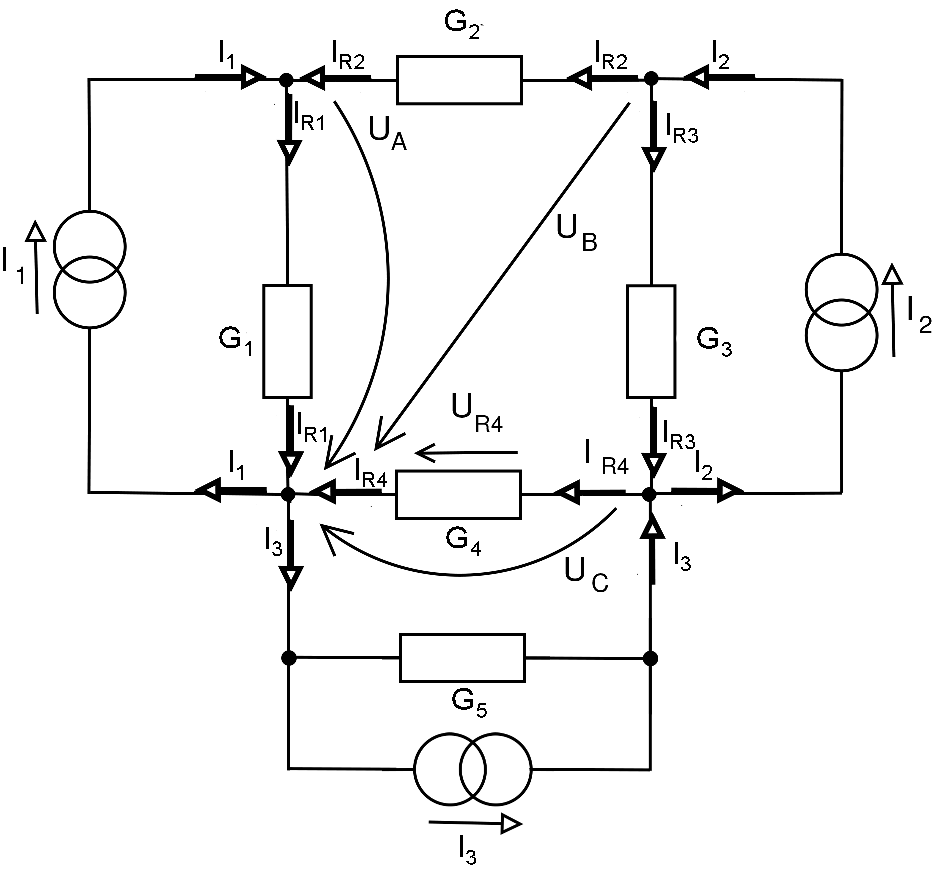
\includegraphics[scale=0.5,keepaspectratio]{sablona/fig/Pr3_Smer_proudovy_vodivost.pdf} \\
    \caption{Převod napěťového zdroje na proudový, odpor na vodivost a vyznačení proudů}
    \end{figure}
\newpage
Převod odporu $\Omega$ na vodivost S:
$$G_1 = \frac{1}{R_1} = \frac{1}{52}S$$
$$G_2 = \frac{1}{R_2} = \frac{1}{42}S$$
$$G_3 = \frac{1}{R_3} = \frac{1}{52}S$$
$$G_4 = \frac{1}{R_4} = \frac{1}{42}S$$
$$G_5 = \frac{1}{R_5} = \frac{1}{21}S$$
\newline
Převod napěťového zdroje U na proudový $I_3$:
$$I_3 = \frac{U}{R_5} = \frac{135}{21} = 6,428571429A$$
\newline
Sestavíme obecné rovnice pro jednotlivé uzly:
$$A: U_A(G_1+G_2) + U_B(-G_2) + U_C(0) = I_1$$
$$B: U_A(-G_2) + U_B(G_2+G_3) + U_C(-G_3) = I_2$$
$$C: U_A(0) + U_B(-G_3) + U_C(G_3 + G_4 + G_5) = I_3 - I_2$$
\newline
Dosadíme do hodnoty do rovnic:
$$A: U_A(\frac{1}{52}+\frac{1}{42}) + U_B(-\frac{1}{42}) + U_C(0) = 0,55$$
$$B: U_A(-\frac{1}{42}) + U_B(\frac{1}{42}+\frac{1}{52}) + U_C(-\frac{1}{52}) = 0,65$$
$$C: U_A(0) + U_B(-\frac{1}{52}) + U_C(\frac{1}{52}+\frac{1}{42}+\frac{1}{21}) = \frac{135}{21} - 0,65$$
\newline
Přepíšeme rovnice do matic:
\[
\left(
\begin{array}{ccc}
\frac{1}{52}+\frac{1}{42} & -\frac{1}{42} & 0\\
-\frac{1}{42} & \frac{1}{42}+\frac{1}{52} & -\frac{1}{52}\\
0 & -\frac{1}{52} & \frac{1}{52}+\frac{1}{42}+\frac{1}{21}\\
\end{array}
\right)
*
\left(
\begin{array}{c}
U_A\\
U_B\\
U_C\\
\end{array}
\right)
=
\left(
\begin{array}{c}
0,55\\
0,65\\
\frac{135}{21}-0,65\\
\end{array}
\right)
\]
\newpage
Vypočítáme determinanty využitím Sarrusového pravidla pro výpočet determinantů:
\[
D = 
\left|
\begin{array}{ccc}
\frac{1}{52}+\frac{1}{42} & -\frac{1}{42} & 0\\
-\frac{1}{42} & \frac{1}{42}+\frac{1}{52} & -\frac{1}{52}\\
0 & -\frac{1}{52} & \frac{1}{52}+\frac{1}{42}+\frac{1}{21}\\
\end{array}
\right|
 = \frac{24299}{144685632}-(\frac{47}{2952768}+\frac{11}{214032})
 = \frac{5}{49686}
\]
\newline
\[
D_3 = 
\left|
\begin{array}{ccc}
\frac{1}{52}+\frac{1}{42} & -\frac{1}{42} & 0,55\\
-\frac{1}{42} & \frac{1}{42}+\frac{1}{52} & 0,65\\
0 & -\frac{1}{52} & \frac{135}{21}-0,65\\
\end{array}
\right|
 = \frac{1787081}{166944960}+\frac{11}{43680}-(-\frac{47}{87360}+\frac{809}{246960})
 = \frac{8167}{993720}
\]
\newline
Využitím Cramerova pravidla (determinant rozšířené matice vydělíme determinantem původní matice):
$$U_C = U_{R_4} = \frac{D_3}{D} = \frac{\frac{8167}{993720}}{\frac{5}{49686}} = \frac{8167}{100} = \mathbf{81,67V}$$
\newline
Využitím Ohmovy metody dopočítáme proud:
$$I_{R_4} = \frac{U_{R_4}}{R_4} = \frac{81,67}{42} = \mathbf{1,94452381A}$$